\section*{Sheet 1}
\subsection*{Exercise 1}
\boldmath
\textbf{A graph is \textit{connected} if, for any vertices $u, v \in V(G), G$ contains a $u - v$ path.\\
Prove that a graph or its complement is connected, possibly both.}\vspace{10pt}\\
\unboldmath
To solve the exercise we will just provide two different proofs, the first one is the following:\vspace{5pt}\\
\boldmath
\textbf{$G$ disconnected $\implies$ $G'$ connected}\vspace{5pt}\\
\unboldmath
If we make the assumption that the graph $G$ is disconnected, then $G$ contains at least two connected components.\\
If we now build the complementary graph to $G$, $G'$, we will have an edge $\forall v, u : v \in V(A) \land u \in V(B)$; where $A$ and $B$ are actually the two connected components we were talking about earlier.\\
Since we are saying that we will have an edge between any two pairs of vertices in $V(G)$ then we are saying that $G'$ is actually connected (the most basic form of connection because we have an actual edge between every single pair).
\vspace{2pt}\\\hspace*{3cm}$\square$\vspace*{10pt}\\
\boldmath
\textbf{$G$ connected $\implies G'$ connected $\vee\hspace{3pt} G'$ disconnected}\vspace{5pt}\\
\unboldmath
To prove this second point we will use counterexamples. \\
\begin{center}
    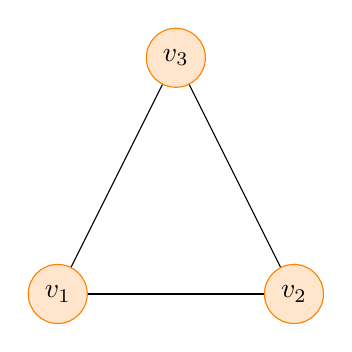
\begin{tikzpicture}
    \tikzset{
    dep/.style={circle,minimum size=0.75cm,fill=orange!20,draw=orange},
    c1/.style={-},
    c2/.style={dotted, red, line width=2},
    }
    \node[dep] (n1) at (0,0) {$v_1$};
    \node[dep] (n2) at (3,0) {$v_2$};
    \node[dep] (n3) at (1.5,3) {$v_3$}; 

    \draw[c1] (n1) edge node[above] {} (n2);
    \draw[c1] (n1) edge node[above] {} (n3);
    \draw[c1] (n2) edge node[above] {} (n3);
\end{tikzpicture}   
\hspace*{3cm}
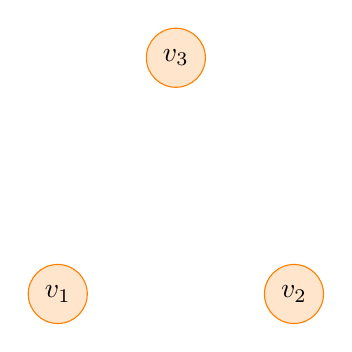
\begin{tikzpicture}
    \tikzset{
    dep/.style={circle,minimum size=0.75cm,fill=orange!20,draw=orange},
    c1/.style={-},
    c2/.style={dotted, red, line width=2},
    }
    \node[dep] (n1) at (0,0) {$v_1$};
    \node[dep] (n2) at (3,0) {$v_2$};
    \node[dep] (n3) at (1.5,3) {$v_3$}; 
\end{tikzpicture}  
\end{center}
In the case above we start with a connected graph and we get a disconnected complementary graph.\vspace{15pt}\\
\begin{center}
    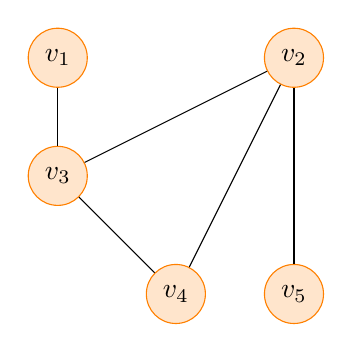
\begin{tikzpicture}
    \tikzset{
    dep/.style={circle,minimum size=0.75cm,fill=orange!20,draw=orange},
    c1/.style={-},
    c2/.style={dotted, red, line width=2},
    }
    \node[dep] (n1) at (0,0) {$v_1$};
    \node[dep] (n2) at (3,0) {$v_2$};
    \node[dep] (n3) at (0,-1.5) {$v_3$}; 
    \node[dep] (n4) at (1.5,-3) {$v_4$};
    \node[dep] (n5) at (3,-3) {$v_5$}; 

    \draw[c1] (n1) edge node[above] {} (n3);
    \draw[c1] (n2) edge node[above] {} (n3);
    \draw[c1] (n3) edge node[above] {} (n4);
    \draw[c1] (n2) edge node[above] {} (n5);
    \draw[c1] (n4) edge node[above] {} (n2);
\end{tikzpicture}   
\hspace*{3cm}
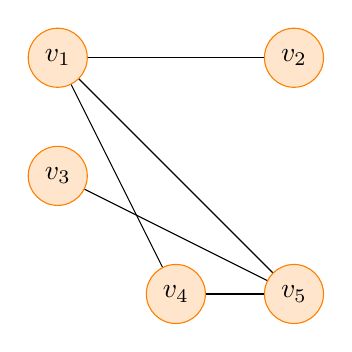
\begin{tikzpicture}
    \tikzset{
    dep/.style={circle,minimum size=0.75cm,fill=orange!20,draw=orange},
    c1/.style={-},
    c2/.style={dotted, red, line width=2},
    }
    \node[dep] (n1) at (0,0) {$v_1$};
    \node[dep] (n2) at (3,0) {$v_2$};
    \node[dep] (n3) at (0,-1.5) {$v_3$}; 
    \node[dep] (n4) at (1.5,-3) {$v_4$};
    \node[dep] (n5) at (3,-3) {$v_5$}; 
    
    \draw[c1] (n1) edge node[above] {} (n2);
    \draw[c1] (n1) edge node[above] {} (n4);
    \draw[c1] (n1) edge node[above] {} (n5);
    \draw[c1] (n3) edge node[above] {} (n5);
    \draw[c1] (n4) edge node[above] {} (n5);
\end{tikzpicture}  
\end{center}
It is perfectly clear that, while the starting graph is connected, the complementary is still connected itself.